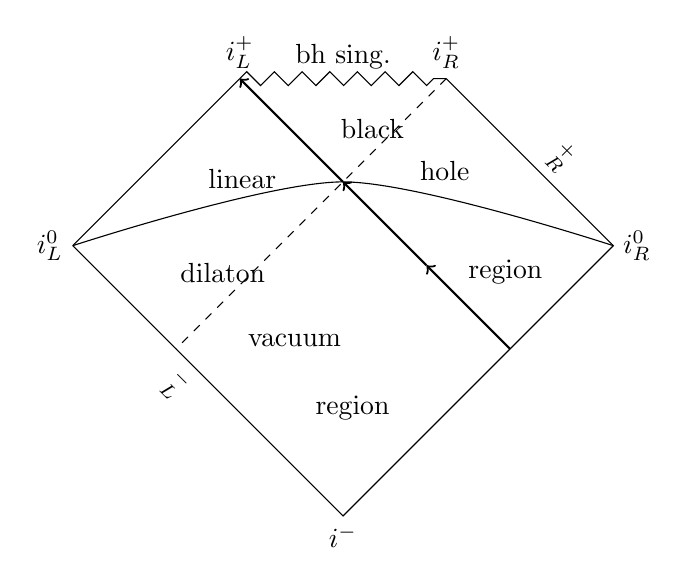
\begin{tikzpicture}%[scale=2]
\pgfmathsetmacro\myunit{3}
\pgfmathsetmacro\grs{0.6180339887498949}
\pgfmathsetmacro\grb{1.6180339887498949}
	\draw (0,0)
			node [left] {$i^0_\text{L}$}
		-- ++ (- 45: \grb * \myunit)
			node [pos = .50, below left, sloped] {$\mscrI^-_\text{L}$}
			node [pos = .10, right = .3*\myunit cm] {dilaton}
			node [pos = .35, right = .3*\myunit cm] {vacuum}
			node [pos = .60, right = .3*\myunit cm] {region}
			node [below] {$i^-$}
		-- ++ (+ 45: \myunit)
			%node [above = .25*\myunit cm] {region}
			coordinate (one)
		-- ++ (+ 45: \grs * \myunit)
			node [pos = .75, left = .15*\myunit cm] {region}
			node [right] {$i^0_\text{R}$}
			coordinate (r-inf)
		-- ++ (+135: \myunit)
			node [pos = .70, left = .35*\myunit cm] {black}
			node [pos = .45, left = .25*\myunit cm] {hole}
 			node [pos = .50, above right, sloped] {$\mscrI^+_\text{R}$}
			node [above] {$i^+_\text{R}$}
			coordinate (r-i+)
			;

	\draw (0,0)
		-- ++ (+ 45: \myunit)
			node [pos = .4, right = .25*\myunit cm] {linear}
			node [above] {$i^+_\text{L}$}
			coordinate (l-i+);
			%node [below = .55*\myunit cm] {linear}
			%node [below = .75*\myunit cm] {dilaton}
			%node [below = .95*\myunit cm] {vacuum};

	\draw [dashed] (r-i+)
		-- ++ (-135: \grb * \myunit)
			coordinate (mlambda);
		
	\draw [thick, ->] (one)
		-- ++ (+135: 0.5 * \myunit)
			coordinate (bb);
	\draw [thick, ->] (bb)
		-- ++ (+135: 0.5 * \myunit)
			coordinate (cross);
	\draw [thick, ->] (cross) -- (l-i+);

	\draw [decorate, decoration=zigzag] (l-i+)
		-- (r-i+)
		node [pos = .5, above] {bh sing.};

	\draw plot [smooth, dash dot] coordinates {(0,0) (cross) (r-inf)};
\end{tikzpicture}